\documentclass[12pt,a4paper]{article}
\usepackage{t1enc}
\usepackage{array}
\usepackage{listings}
\usepackage{color}
\usepackage[table]{xcolor}
\usepackage{graphicx}
\usepackage{float}
\usepackage{hyperref}
\usepackage{geometry}
\usepackage[hungarian]{babel}

\geometry{
    a4paper,
    left=25mm,
    right=25mm,
    top=25mm,
    bottom=25mm
}

\hypersetup{
    colorlinks=true,
    linkcolor=blue,
    citecolor=black,
    filecolor=black,
    urlcolor=blue,
    pdfborder={0 0 0}
}

\pagenumbering{gobble}

\setcounter{secnumdepth}{0}

\begin{document}

% Cover Page
\begin{titlepage}
    \centering
    \vspace*{\fill}
    \textbf{\Huge Silicon Labs HackathON}\\[1cm]
    \textbf{\Large Okosotthon, de mi van ha Te vagy az okosabb}\\[2cm]
    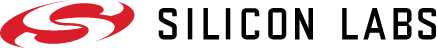
\includegraphics[width=0.65\textwidth]{figures/silabs-logo.png}\\[2cm]
    \textbf{\Large THERMOnkey}\\[0.5cm]
    \Large Az okos hőmérsékleti megoldás.\\[2cm]
    \Large \textbf{\textit{Csapattagok:}}\\[0.25cm]
    \Large Csuta Krisztián, Kovács Levente, Mészáros Bálint\\[0.25cm]
    Villamosmérnök BSc\\
    Budapesti Műszaki és Gazdaságtudományi Egyetem\\[2cm]
    \Large \today
    \vspace*{\fill}
\end{titlepage}

\newpage

\pagenumbering{arabic}

\section{Projekt bemutatása}

A THERMOnkey egy okos hőmérséklet-figyelő, illetve szabályozó rendszer, amely vezeték nélküli kommunikációval képes adatokat továbbítani és megjeleníteni.
A projekt célja egy könnyen használható, megbízható és bővíthető megoldás létrehozása volt, amely otthoni vagy akár ipari környezetben is alkalmazható.
A projekt GitHub repositoryja ide kattintva érhető el: \href{https://github.com/tuskeshatu/silabs-thermonkey}{https://github.com/tuskeshatu/silabs-thermonkey}.

\section{Rendszer felépítése}

\subsection{Okosotthon-képes termosztát vezérlőegység}
A vezérlőegységet egy \textbf{MG24 dev-kit} segítségével valósítottuk meg. 

\subsubsection{Matter és okosotthon?}
A rendszer egyik fő előnye, hogy könnyedén integrálható különböző okosotthon platformokkal, a \textbf{Matter over Thread} protokoll támogatásával.
Ezt szoftveresen a Silabs Arduino core-ba integrált Matter API segítségével könnyedén megvalósíthattuk. Az eszközt indításkor commission-ölni kell egy
Matter hálózatba, utána pedig intuitívan és egyszerűen, akár távolról is vezérelhető (mint bármilyen egyéb okosotthon képes termosztát). Mi ennek a tesztelését
Apple home környezetben valósítottuk meg.

\begin{figure}[H]
    \centering
    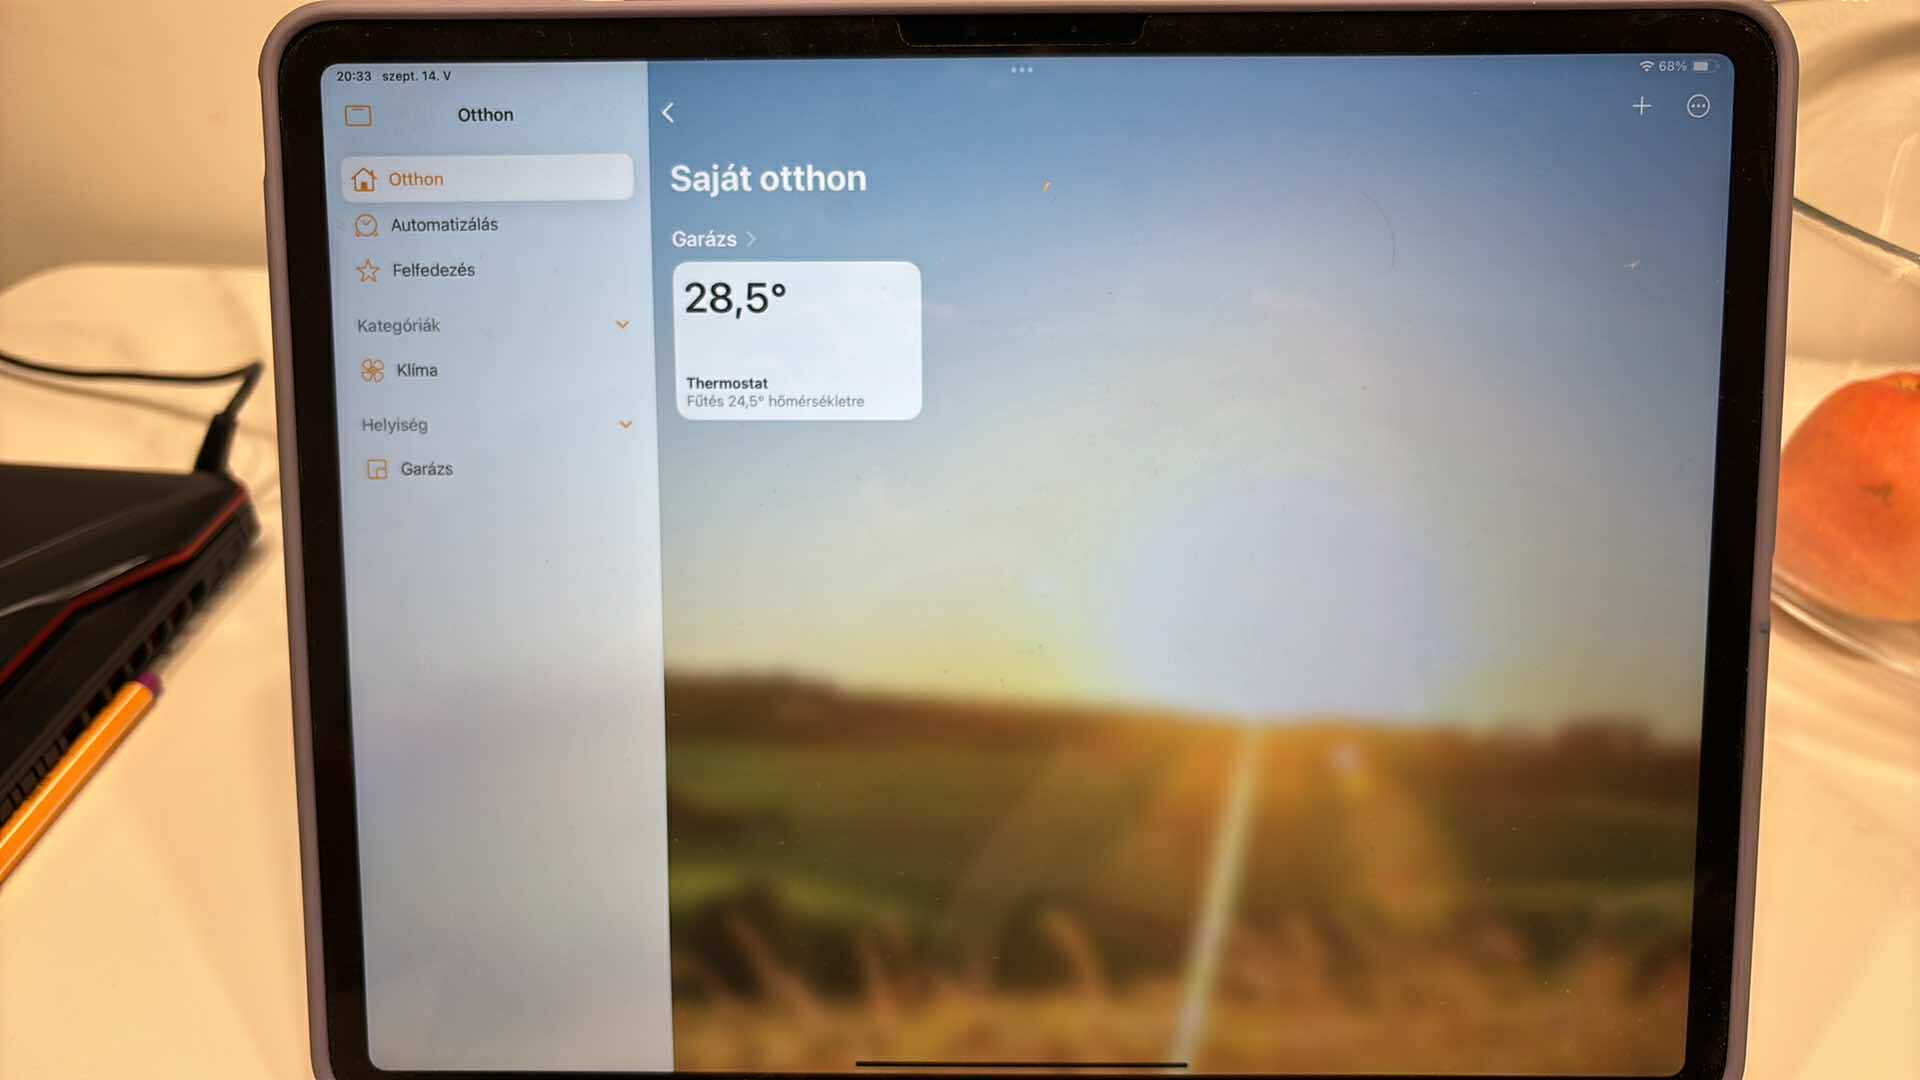
\includegraphics[width=0.8\textwidth]{figures/apple__home.jpg}
    \caption{Apple home környezetben a THERmonkey termosztát}
    \label{fig:rirs}
\end{figure}

\pagebreak

\subsubsection{Ház és kijelző}
\begin{minipage}{0.65\textwidth}
A falra szerelhető, 3D nyomtatott dobozban helyet kapott egy \textbf{Adafruit 0.96" 160x80 Color TFT} kijelző, melyen kezdetkor megjelenik a Matter párosításhoz
szükséges kód. Ez elengedhetetlen a felhasználóbarát működéshez. Miután a termosztát integrálva lett egy okosotthon környezetbe, a képernyő felváltva a
fejlesztőboard \textbf{beépített szenzorja által mért}, jelenlegi hőmérsékletet, illetve a Matter-ön keresztül kapott beállított hőmérsékletet írja ki.
A megjelenítéshez a kijelzőhöz tartotó Arduino library-t használtuk \textit{(megj.: ez egyáltalán nem bizonyult intuitívnak, vagy egyszerűnek)}.
\end{minipage}
\hfill
\begin{minipage}{0.3\textwidth}
    \centering
    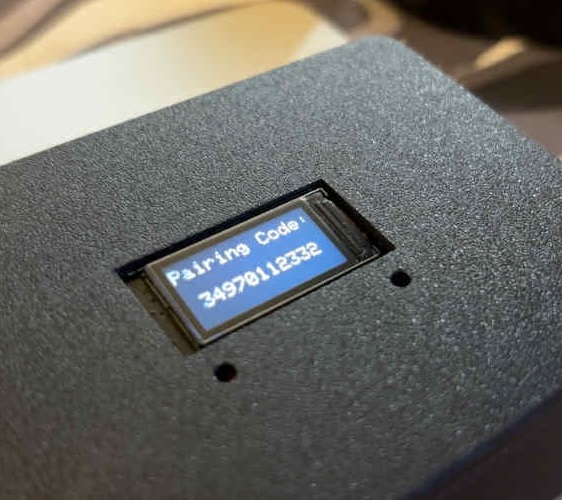
\includegraphics[width=\textwidth]{figures/pairing-code.jpg}
    %\vspace{0.15cm}
\end{minipage}

\begin{figure}[H]
    \centering
    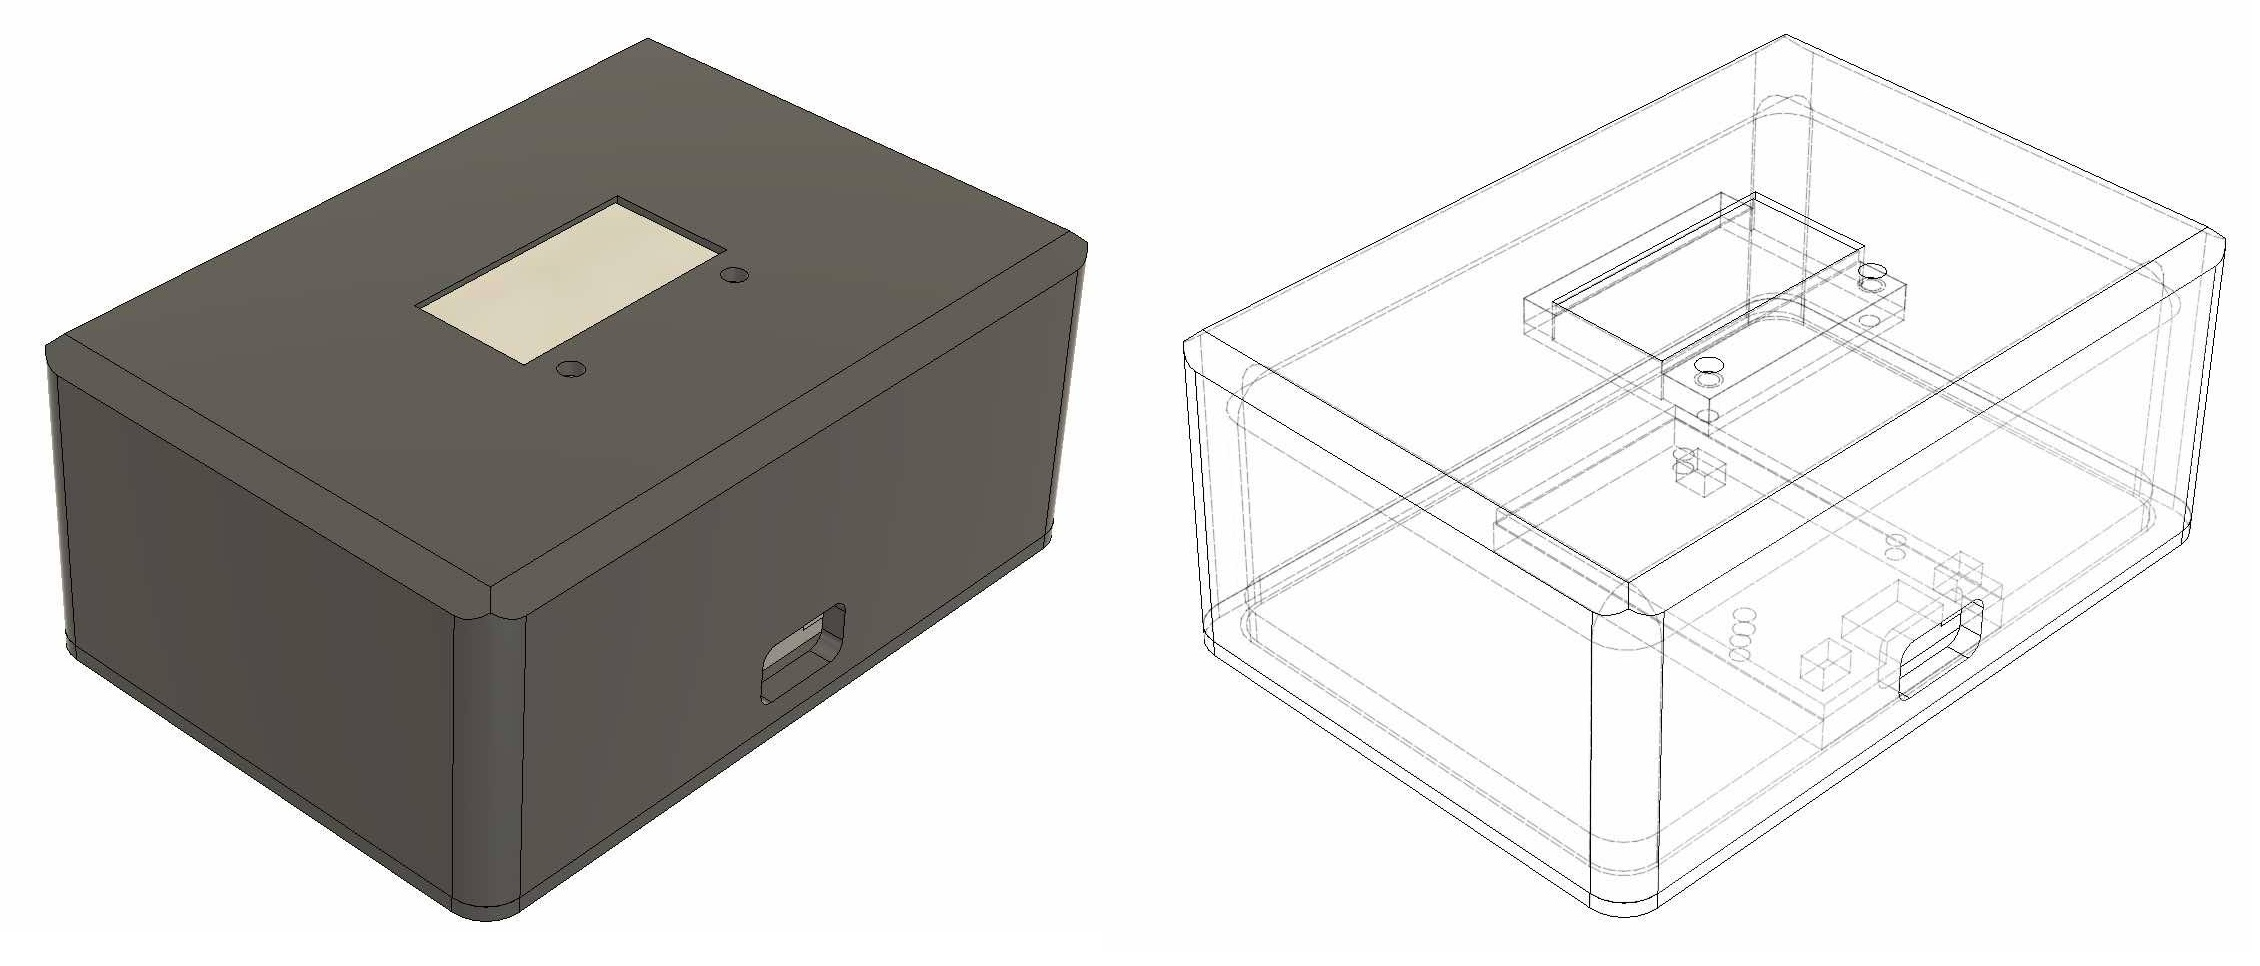
\includegraphics[width=0.8\textwidth]{figures/termosztat-haz.jpg}
    \caption{A termosztát ház 3D modellje}
    \label{fig:rirs}
\end{figure}

\subsection{Hőmérsékletszabályozást megvalósító vezeték nélküli termofej}
\begin{minipage}{0.65\textwidth}
A termofejet a \textbf{MG24 explorer-kit} boardja hajtja meg. Ezeknek a végső radiátorra szerelhetősége két problémát vet fel: az egyik az áramellátás,
a másik a vezérléshez szükséges információátadás.
\end{minipage}
\hfill
\begin{minipage}{0.3\textwidth}
    \centering
    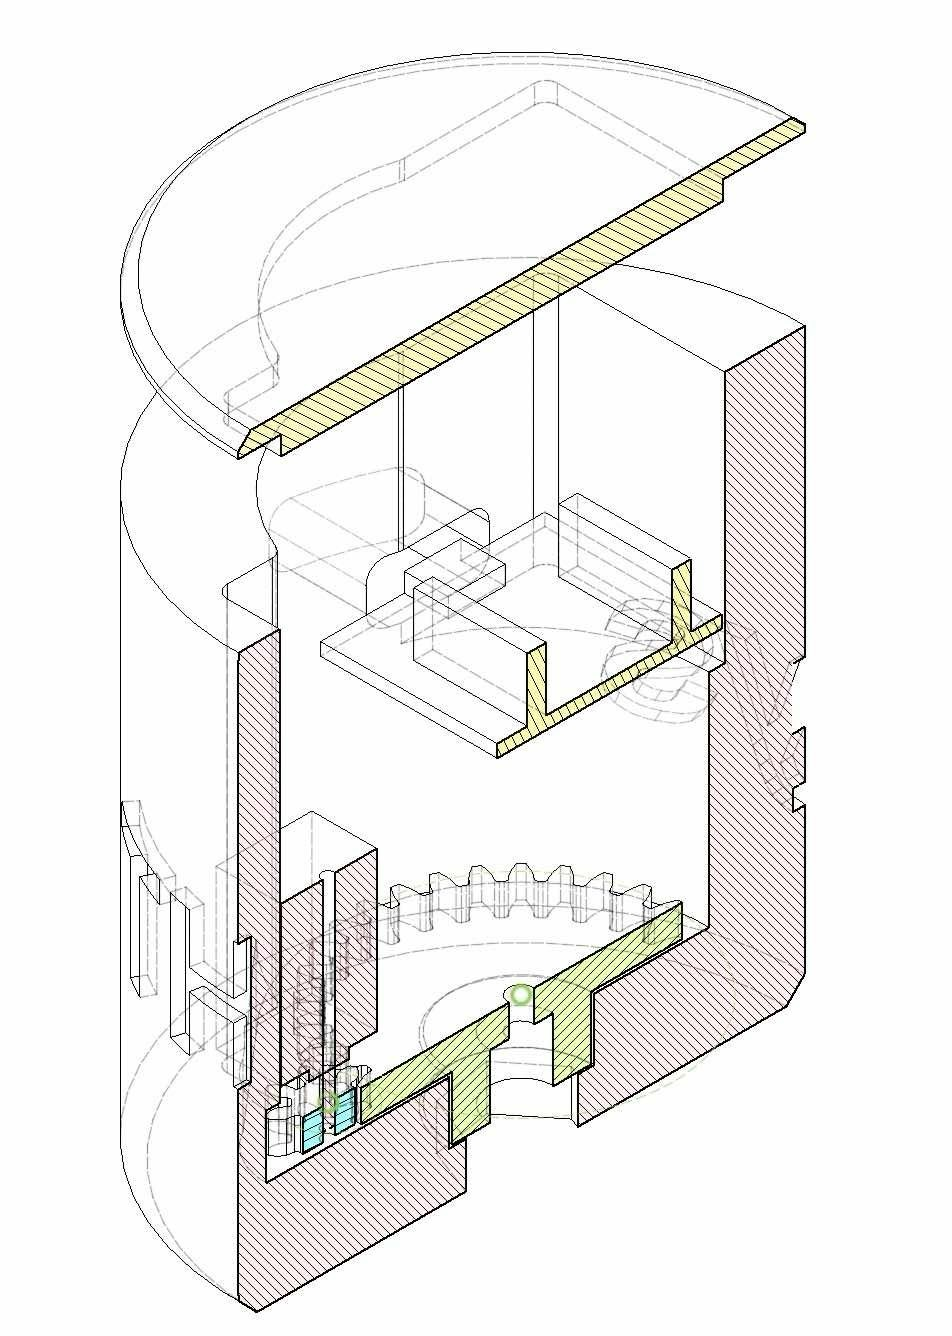
\includegraphics[width=\textwidth]{figures/termofej.jpg}
    %\vspace{0.15cm}
\end{minipage}

\subsubsection{Áramellátás}
Az eredeti tervek szerint az áramellátást egy lecsatlakoztatható akkumulátorral oldottuk volna meg, ám realizáltuk, hogy custom akkumulátorpakkok nélkül a limitált méret
miatt ez fizikai képtelenség lenne. A végső megoldásunkban 4db 1.5 V-os, AA-s elem került beépítésre a házba.

Annak érdekében, hogy az eszköz minél lasabban merüljön, drasztikus fogyasztáscsökkentést kellett elérnünk. Az alábbi táblázatban láthatóak az elérhető nagyszerű és az
Arduino Low Power library segítségével egyszerűen vezérelhető energia állapotai a boardnak.

\begin{table}[h!]
\centering
\renewcommand{\arraystretch}{1.4}
\begin{tabular}{|>{\raggedright\arraybackslash}p{2cm}|
                >{\raggedright\arraybackslash}p{8cm}|
                >{\raggedright\arraybackslash}p{3cm}|}
\hline
\rowcolor{lightgray}
\textbf{Energy Mode} & \textbf{Description} & \textbf{Power Consumption} \\
\hline
EM0 -- Run & CPU aktív, utasításokat hajt végre Flash-ből vagy RAM-ból; minden alacsony energia periféria engedélyezhető. & 180 $\mu$A/MHz \\
\hline
EM1 -- Sleep & CPU órajel leáll, de RAM és perifériák működnek; PRS és DMA révén CPU beavatkozás nélkül dolgozhat. & 45 $\mu$A/MHz \\
\hline
EM2 -- Deep Sleep & Nagyfrekvenciás oszcillátor kikapcsolva, de 32 kHz óra és RTC elérhető; CPU nem fut, RAM megtartva. & 0.9 $\mu$A \\
\hline
EM3 -- Stop & Alacsony frekvenciás oszcillátor kikapcsolva; RAM megtartva; analóg komparátor vagy külső megszakítás ébreszthet. & 0.6 $\mu$A \\
\hline
\rowcolor{lightgray}
\textbf{EM4 -- Shutoff} & \textbf{MCU teljesen leáll; nincs RTC vagy RAM megtartás. Csak reset vagy külső megszakítás ébreszti.} & \textbf{20 nA} \\
\hline
\end{tabular}
\caption{EFM32 energia módok összehasonlítása (kiemelve az EM4 tulajdonságai).}
\end{table}

Ezek alapján egyértelműen látszik, hogy miért választottuk a szinte teljes kikapcsolását a boardnak. Mivel egy szonának a hőtehetetlensége szerencsére elég nagy, ezért
szoftverben egyszerűen vezérelhető módon úgy programoztuk ezeket, hogy csak időnként ébredjenek fel, kérdezzék meg a termosztátot, hogy hány fok van és mennyinek kéne
lennie, majd visszaalszanak \textbf{(, vagyis sleepy end deviceok)}. Ezzel sikerült elérni, hogy gyakorlatilag amikor nem történik aktív vezérlés, akkor nincs áramfogyasztás sem.

\subsubsection{Vezeték nélküli kommunikáció}
A fentebb említett energiafelhasználási megkötések és az egyszerűség kedvéért a megoldásunk Bluetooth Low Energy (BLE) technológiát használ a termosztát és a termofejek közötti
kommunikációra. A termosztát egy always-on BLE szerverként viselkedik, amire az éppen aktuálisan felébredő termofej kliensként felcsatlakozik, majd miután megkapta a hőmérsékleti
adatokat elmegy alacsony fogyasztású üzemmódba. Amennyiben egy ideig nem sikerült a termofejnek csatlakozni a BLE szerverhez (termosztáthoz), abban az esetben timeout-ol és szintén
visszamegy aludni. Fontos, hogy a timeout időt megfelelően hosszúra válasszuk, hogy mindegyik termofej sorra kerüljön.

\subsubsection{Mechanikai megoldások}
A radiátoron található csavar elcsavarásához szükséges viszonylag nagy nyomaték miatt a designban helyet kapott egy 1:4 áttétű fogaskerék rendszer is.
Egy \textbf{Adafruit MOSFET Driverrel} meghajtott DC motor tengelye csatlakozik a kisebb fogaskerékre, míg a nagyobb fogaskerék közvetlenül ráilleszthető
a standard csavarra a radiátoron.

\begin{figure}[H]
    \centering
    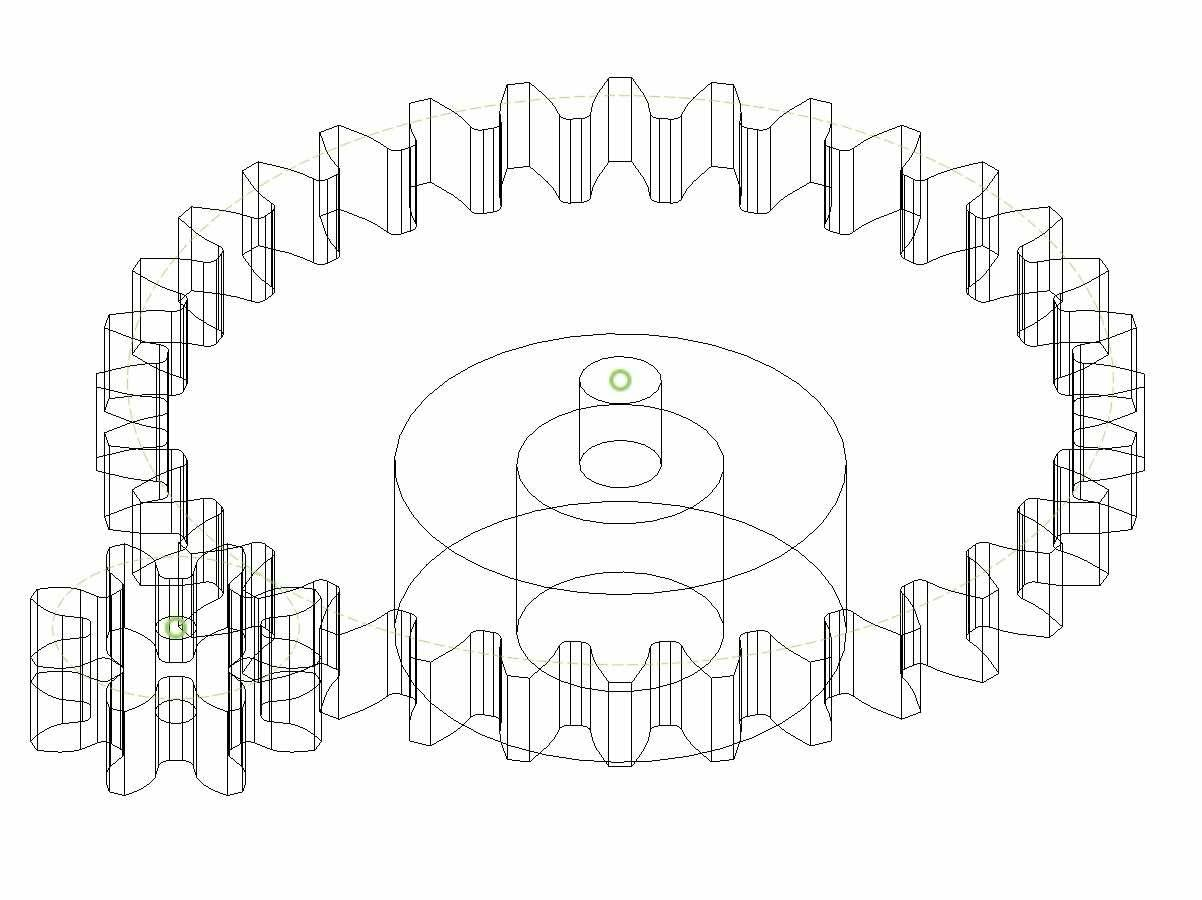
\includegraphics[width=0.8\textwidth]{figures/fogaskerek.jpg}
    \caption{A fogaskerekek (1:4 áttét)}
    \label{fig:rirs}
\end{figure}

\newpage

\section{Amire a legbüszkébbek vagyunk}

Különösen büszkék vagyunk arra, hogy sikerült stabil és megbízható Matter és BLE kommunikációt kialakítani.
Mivel a Matter is használja a BLE stacket és funkcionalitásokat, ezért a két funkcionalitás (termofej-termosztát és termosztát-Matter hub kommunikáció) együttes, egymást nem
zavaró és kizáró megvalósítása nem volt egyszerű feladat.

A rendszer energiahatékonysága és az ezzel összeegyeztethetetlen (kis méret, vezeték nélküliség) követelmények az eszköz iránt is kiemelkedően sok fejvakarást okoztak.
Az alacsony energiafogyasztású állapotban mivel szinte semmilyen periféria nem működik, ezért egy működőképes konstrukció kitalálása az okosotthonba integrálhatósághoz 
nehéz feladat.

A különböző perifériák kezelése közül külön említést érdemel az Adafruit 0.96" 160x80 Color TFT kijelző, melynek a könyvtára által adott édes lehetőségek tengere annyira
elárasztott bennünket, hogy a kód kellemetlenül nagy részét kiteszi a megjelenítés. Jónéhány sor \textbf{csak} azért felel, hogy a ° karaktert megjelenítsük.

Összességében a projekt során nemcsak szakmai tudásunkat bővítettük, hanem megtapasztaltuk a \textit{közös munka örömét} és a \textit{problémamegoldás izgalmát} is.
A végeredmény egy működő, hasznos és (mind szoftveresen és hardveresen) egyszerűen bővíthető rendszer lett, amelyre mindannyian büszkék vagyunk.

\end{document}